\section{Trendy}
\label{sec:trendy}

\subsection{Trend Big Data}
\label{sub:trend_big_data}
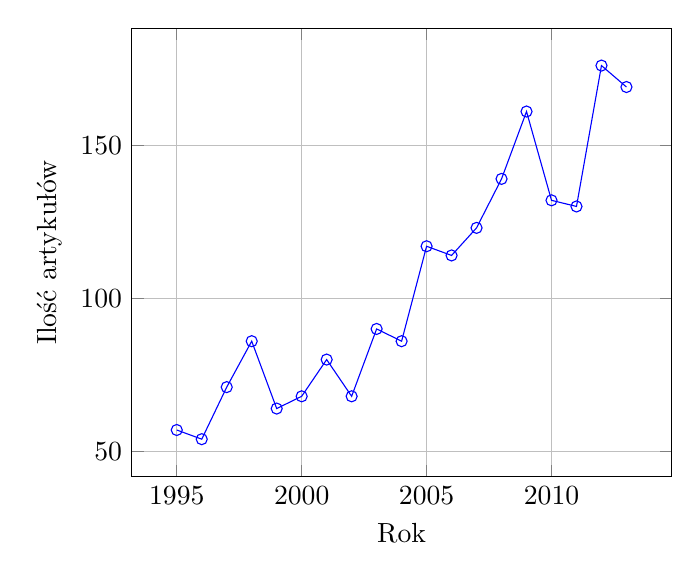
\begin{tikzpicture}
    \begin{axis}[
            xlabel=Rok,
            ylabel=Ilość artykułów,
            /pgf/number format/.cd,
            use comma,
            grid=major,
            1000 sep={}
        ]
        \addplot[color=blue, mark=o] coordinates {
            (1995, 57) 
            (1996, 54) 
            (1997, 71) 
            (1998, 86) 
            (1999, 64) 
            (2000, 68) 
            (2001, 80) 
            (2002, 68) 
            (2003, 90) 
            (2004, 86) 
            (2005, 117) 
            (2006, 114) 
            (2007, 123) 
            (2008, 139) 
            (2009, 161) 
            (2010, 132) 
            (2011, 130) 
            (2012, 176) 
            (2013, 169) 
        };
    \end{axis}
\end{tikzpicture}

% section trendy (end)
